% Chapter 11 -- Multivariable calculus: gradients, Jacobians, Hessians
\chapter{Multivariable calculus: gradients, Jacobians, Hessians}\label{ch:mvcalc}

Every loss function you will ever minimize is a scalar field over many
variables --- and every optimizer reads its gradient. This chapter gives
you the three derivative objects you actually need: the gradient (vector
of steepest ascent), the Jacobian (the local linear map), and the Hessian
(the curvature), plus the matrix-form chain rule that makes backprop
nothing more than disciplined matrix multiplication. After this chapter
you can derive $\nabla_{\mathbf x}\mathbf x^{T}A\mathbf x=(A+A^{T})\mathbf
x$ by hand, check any gradient with finite differences in three lines of
code, and read a Jacobian as a local grid warp.

\section{Partial derivatives}\label{sec:mvc-partials}

For $f:\mathbb R^{n}\to\mathbb R$, the \emph{partial
derivative}\index{partial derivative} $\partial f/\partial x_i$ is the
ordinary derivative in coordinate $i$, all other variables frozen:
\[
\frac{\partial f}{\partial x_i}(\mathbf x_0)=\lim_{h\to0}
\frac{f(\mathbf x_0+h\mathbf e_i)-f(\mathbf x_0)}{h}.
\]
No new mechanics --- just $n$ ordinary derivatives, one per axis. The
subtlety is what they measure: each is a slope along an axis, and a
function needs more than axis-wise good behaviour to be well-behaved
(differentiability is existence of the linear approximation of
Section~\ref{sec:mvc-jacobian}, not merely of partials).

\section{The gradient and the steepest direction}\label{sec:mvc-grad}

\begin{definition}[Gradient]\index{gradient}
The \emph{gradient} of $f$ at $\mathbf x$ is the column vector of
partials:
\[
\nabla f(\mathbf x)=\begin{bmatrix}\partial f/\partial x_1\\ \vdots\\
\partial f/\partial x_n\end{bmatrix}.
\]
It is the unique vector such that
$f(\mathbf x_0+\Delta)\approx f(\mathbf x_0)+\nabla f\cdot\Delta$.
\end{definition}

The directional derivative\index{directional derivative} along unit
$\mathbf d$ is $\nabla f\cdot\mathbf d=\lVert\nabla f\rVert\cos\theta$,
maximized when $\mathbf d\parallel\nabla f$ --- the gradient really IS
the direction of steepest ascent, and its norm is the steepest slope
(Figure~\ref{fig:dirderiv}). It is also everywhere normal to the level
sets (Figure~\ref{fig:gradcontour}): the tangent direction $\mathbf t$
satisfies $\nabla f\cdot\mathbf t=0$.

\begin{figure}[htbp]
\centering
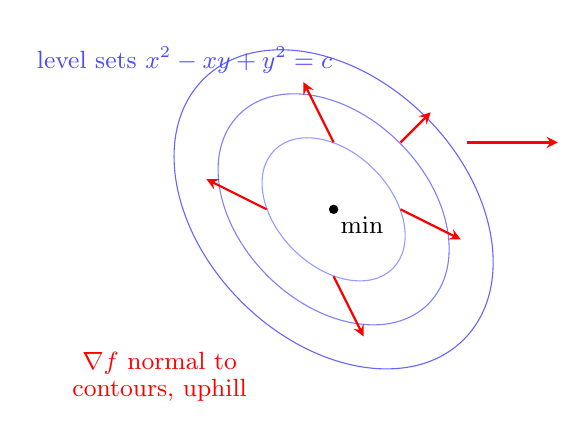
\begin{tikzpicture}[scale=0.85,>=stealth]
% f = x^2 - xy + y^2 level sets are ellipses rotated 45deg: f = (x^2+y^2)/2 in rotated coords ~ radius sqrt(2c/3) and sqrt(2c)
\begin{scope}[rotate=45]
\draw[blue!40] (0,0) ellipse (0.85 and 1.25);
\draw[blue!50] (0,0) ellipse (1.4 and 2.0);
\draw[blue!60] (0,0) ellipse (1.95 and 2.75);
\node[blue!70] at (0,3.15) {\small level sets $x^2-xy+y^2=c$};
\end{scope}
% arrows: (1,0)->(2,-1), (0,1)->(-1,2), (1,1)->(1,1), (-1,0)->(-2,1), (0,-1)->(1,-2), scaled 0.45
\draw[->,red,thick] (1,0)--(1.9,-0.45);
\draw[->,red,thick] (0,1)--(-0.45,1.9);
\draw[->,red,thick] (1,1)--(1.45,1.45);
\draw[->,red,thick] (-1,0)--(-1.9,0.45);
\draw[->,red,thick] (0,-1)--(0.45,-1.9);
\draw[->,red,thick] (2,1)--(3.35,1.0);
\fill (0,0) circle (2pt) node[below right=-1pt]{\small min};
\node[red] at (-2.6,-2.3) {\small $\nabla f$ normal to};
\node[red] at (-2.6,-2.7) {\small contours, uphill};
\end{tikzpicture}

\caption{Gradient field over level sets of $f=x^{2}-xy+y^{2}$ (real
samples from \ttfamily code/ch11\_grad\_field.py). Notice every arrow is
perpendicular to the contour it leaves --- and points uphill.
Regenerate: \ttfamily figures/ch11\_grad\_contour.tex.}
\label{fig:gradcontour}
\end{figure}

\begin{figure}[htbp]
\centering
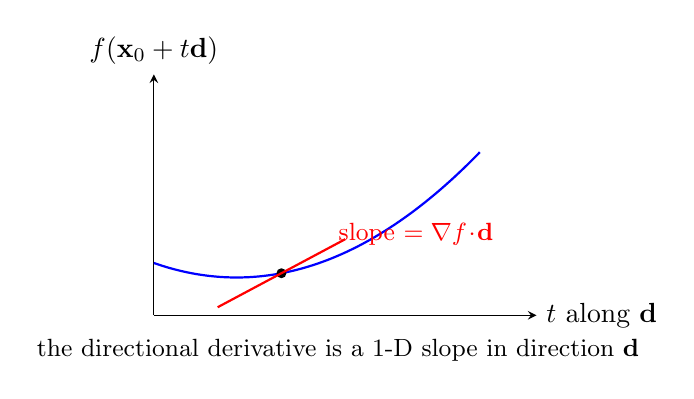
\begin{tikzpicture}[scale=0.9,>=stealth]
\draw[->] (0,0)--(5.4,0) node[right]{$t$ along $\mathbf d$};
\draw[->] (0,0)--(0,3.4) node[above]{$f(\mathbf x_0+t\mathbf d)$};
\draw[domain=0:4.6,smooth,variable=\t,thick,blue] plot (\t,{0.15*(\t-1.5)^2 + 0.1*\t + 0.4});
\fill (1.8,{0.15*0.09 + 0.18 + 0.4}) circle (2pt);
\draw[red,thick] (0.9,{0.5935-0.48})--(2.7,{0.5935+0.48});
\node[red] at (3.7,1.15) {\small slope $=\nabla f\!\cdot\!\mathbf d$};
\node at (2.6,-0.5) {\small the directional derivative is a 1-D slope in direction $\mathbf d$};
\end{tikzpicture}

\caption{A directional derivative is an ordinary slope in a sliced
direction. Notice $\nabla f\cdot\mathbf d$ is maximized when $\mathbf d$
aligns with the gradient. Regenerate:
\ttfamily figures/ch11\_dir\_deriv.tex.}
\label{fig:dirderiv}
\end{figure}

\section{The Jacobian: local linear approximation}\label{sec:mvc-jacobian}

For $\mathbf F:\mathbb R^{n}\to\mathbb R^{m}$ the
\emph{Jacobian}\index{Jacobian} is the $m\times n$ matrix of all
partials: $J_{ij}=\partial F_i/\partial x_j$ --- rows index outputs,
columns index inputs. Then
\[
\mathbf F(\mathbf x_0+\Delta)\approx\mathbf F(\mathbf x_0)+J(\mathbf
x_0)\,\Delta:
\]
the map is locally a matrix --- the whole point of linear algebra, again
(Figure~\ref{fig:jacwarp}). A scalar field's Jacobian is the gradient as
a ROW vector; we store the gradient itself as a column (notation
decision, and a real source of bugs --- Section~\ref{sec:mvc-mistakes}).

\begin{figure}[htbp]
\centering
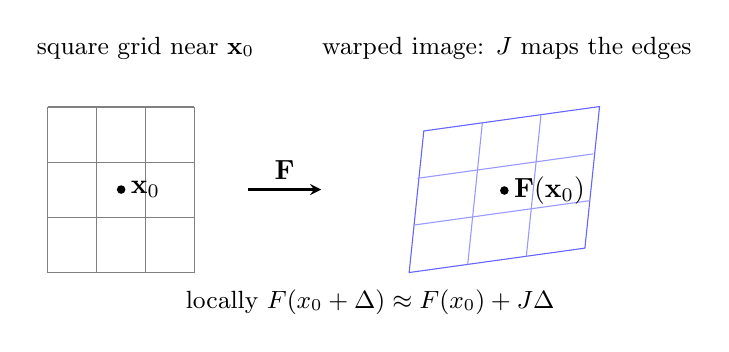
\begin{tikzpicture}[scale=0.62,>=stealth]
\node at (2,4.6) {\small square grid near $\mathbf x_0$};
\foreach \i in {0,1,2,3} \draw[gray] (\i,0)--(\i,3.4);
\foreach \i in {0,1,2,3} \draw[gray] (0,\i*1.13)--(3,\i*1.13);
\fill (1.5,1.7) circle (2.5pt) node[right]{$\mathbf x_0$};
\draw[->,thick] (4.1,1.7)--(5.6,1.7) node[midway,above]{$\mathbf F$};
\begin{scope}[xshift=7.4cm]
\node at (2,4.6) {\small warped image: $J$ maps the edges};
% parallelogram-ish warp
\draw[blue!60] (0,0)--(3.6,0.5)--(3.9,3.4)--(0.3,2.9)--cycle;
\draw[blue!40] (1.2,0.17)--(1.5,3.07);
\draw[blue!40] (2.4,0.33)--(2.7,3.23);
\draw[blue!40] (0.08,0.97)--(3.68,1.47);
\draw[blue!40] (0.17,1.93)--(3.77,2.43);
\fill (1.95,1.68) circle (2.5pt) node[right]{$\mathbf F(\mathbf x_0)$};
\end{scope}
\node at (6.6,-0.6) {\small locally $F(x_0+\Delta)\approx F(x_0)+J\Delta$};
\end{tikzpicture}

\caption{The Jacobian as a local grid warp. Notice the image of the
little grid is (approximately) a parallelogram --- $J$ is the linear map
that sends grid edges to parallelogram edges. Regenerate:
\ttfamily figures/ch11\_jacobian\_warp.tex.}
\label{fig:jacwarp}
\end{figure}

\begin{example}[Jacobian of a vector-valued function]\label{ex:jac}
\textbf{Strategy.} For
$\mathbf F(x,y)=[x^{2}+y,\ \sin x\cdot y,\ x-2y]^{T}$, write the six
partials in output-rows $\times$ input-cols order, then evaluate and
verify numerically.

\textbf{Solution.}
\[
J=\begin{bmatrix}2x & 1\\ y\cos x & \sin x\\ 1 & -2\end{bmatrix},
\qquad
J(0.7,1.2)=\begin{bmatrix}1.4&1\\0.9178&0.6442\\1&-2\end{bmatrix}
\]
matching the finite-difference Jacobian in the listing below to all
printed digits.
\end{example}

\begin{lstlisting}[caption={\ttfamily code/ch11\_wrong\_layout.py --- the
instructive layout bug: transposing the Jacobian produces a $2\times3$
that cannot even act on an input vector.}]
import numpy as np
np.set_printoptions(precision=4, suppress=True)

# f: R^2 -> R^3, Jacobian should be 3x2 (rows=outputs, cols=inputs)
def f(v):
    x, y = v
    return np.array([x*x + y, np.sin(x)*y, x - 2*y])

x0 = np.array([0.7, 1.2])
def jacobian_fd(f, x, h=1e-6):
    m = len(f(x)); n = len(x)
    J = np.zeros((m, n))
    for j in range(n):
        d = np.zeros(n); d[j] = h
        J[:, j] = (f(x + d) - f(x - d)) / (2*h)
    return J

J = jacobian_fd(f, x0)
print("correct Jacobian (3x2):"); print(J)
J_bad = jacobian_fd(f, x0).T   # the classic layout bug
v = np.array([1., 0.])
print("J @ v (right direction) :", J @ v)
try:
    print("J_bad @ v:", J_bad @ v)
except ValueError as e:
    print("J_bad @ v ->", e)
print("J_bad gives a 2x3: applying it to an input vector CRASHES")
\end{lstlisting}

\begin{lstlisting}[caption={Output of the layout bug. Notice the
transposed Jacobian is a $2\times3$ --- the error only fires when you try
to apply it. Layout bugs in gradients are silent precisely where the
shapes happen to agree.}]
correct Jacobian (3x2):
[[ 1.4     1.    ]
 [ 0.9178  0.6442]
 [ 1.     -2.    ]]
J @ v (right direction) : [1.4    0.9178 1.    ]
J_bad @ v -> matmul: Input operand 1 has a mismatch in its core dimension 0, with gufunc signature (n?,k),(k,m?)->(n?,m?) (size 2 is different from 3)
J_bad gives a 2x3: applying it to an input vector CRASHES
\end{lstlisting}

\begin{exercise}[easy]
For $\mathbf F(x,y)=[xy,\ x+y,\ x^{2}]^{T}$ write $J$ and state its
shape. Which row belongs to which output?
\end{exercise}

\section{The Hessian and second-order information}\label{sec:mvc-hess}

The \emph{Hessian}\index{Hessian} $H$ of $f$ is the Jacobian of
$\nabla f$: $H_{ij}=\partial^{2}f/\partial x_i\partial x_j$. For
twice-continuously-differentiable $f$ it is symmetric (Clairaut) ---
chapter 9's whole toolkit applies: eigenvalues of $H$ are principal
curvatures. $H\succ0$ at a critical point $\Rightarrow$ local min;
indefinite $\Rightarrow$ saddle. The Rosenbrock banana
(Figure~\ref{fig:rosen}) is where first-order methods crawl: gradients
shrink along the valley while the curvature says the valley is curved.

\begin{figure}[htbp]
\centering
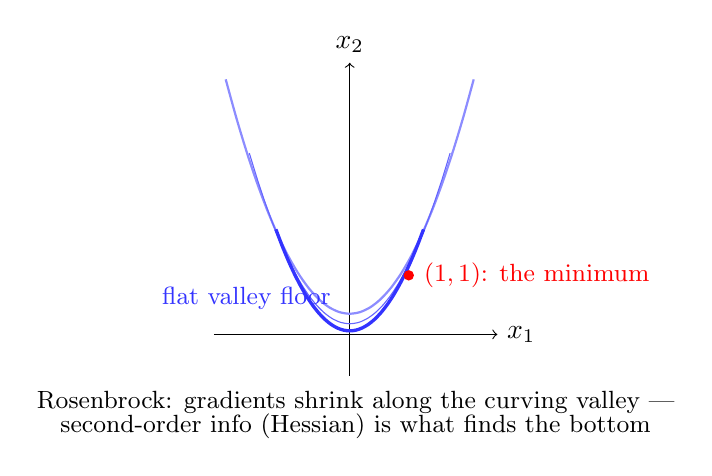
\begin{tikzpicture}[scale=0.75]
% banana valley: x2 = x1^2 curve; contours nested parabola-ish
\draw[->] (-2.3,0)--(2.5,0) node[right]{$x_1$};
\draw[->] (0,-0.7)--(0,4.6) node[above]{$x_2$};
\draw[domain=-2.1:2.1,smooth,variable=\x,blue!45,thick] plot (\x,{0.9*\x*\x+0.35});
\draw[domain=-1.7:1.7,smooth,variable=\x,blue!60] plot (\x,{\x*\x+0.18});
\draw[domain=-1.25:1.25,smooth,variable=\x,blue!80,very thick] plot (\x,{1.1*\x*\x+0.06});
\fill[red] (1,1) circle (2.5pt) node[right=2pt]{\small $(1,1)$: the minimum};
\node[blue!80] at (-1.75,0.62) {\small flat valley floor};
\node at (0.1,-1.15) {\small Rosenbrock: gradients shrink along the curving valley ---};
\node at (0.1,-1.55) {\small second-order info (Hessian) is what finds the bottom};
\end{tikzpicture}

\caption{The Rosenbrock banana valley. Notice the minimum sits on a
nearly-flat curving floor --- first-order info alone can't see around
the bend. Regenerate: \ttfamily figures/ch11\_rosenbrock.tex.}
\label{fig:rosen}
\end{figure}

\section{The chain rule in matrix form (the backprop engine)}\label{sec:mvc-chain}

If $\mathbf y=\mathbf g(\mathbf x)$ and $\mathbf z=\mathbf f(\mathbf
y)$, then
\[
J_{f\circ g}(\mathbf x)=J_f(\mathbf y)\,J_g(\mathbf x):
\]
Jacobians multiply in composition order --- left factor = outer function.
For scalar loss $L=\ell(\mathbf y)$ this reads
$\nabla_{\mathbf x}L=J_g^{T}\nabla_{\mathbf y}L$: gradient flows BACK
through transposed Jacobians. That single line is backpropagation.

\begin{example}[Two-step chain rule in matrix form]\label{ex:chain}
\textbf{Strategy.} $L=\tfrac12\lVert A\mathbf x-\mathbf b\rVert^{2}$ as a
composition: $\mathbf r=A\mathbf x-\mathbf b$ (Jacobian $A$), then
$L=\tfrac12\mathbf r^{T}\mathbf r$ (gradient $\mathbf r$). Multiply in
order.

\textbf{Solution.}
$\nabla_{\mathbf x}L=J_{\mathbf r}^{T}\nabla_{\mathbf r}L
=A^{T}\mathbf r=A^{T}(A\mathbf x-\mathbf b)$ --- the normal-equations
gradient of chapter 8, derived as one chain-rule step instead of a
page of index juggling.
\end{example}

\begin{exercise}[medium]
Chain-rule the two-layer map $\mathbf z=A_2\sigma(A_1\mathbf x+\mathbf
b_1)$ with elementwise $\sigma$: write the full Jacobian
$\mathbf x\mapsto\mathbf z$.
\begin{solution}
$J=A_2\,\operatorname{diag}(\sigma'(A_1\mathbf x+\mathbf b_1))\,A_1$ ---
the diag factor is the per-neuron gate; this IS a two-layer network's
backprop matrix.
\end{solution}
\end{exercise}

\section{Worked library}\label{sec:mvc-library}

Four gradients you will recompute forever:

\begin{center}
\begin{tabularx}{\textwidth}{l>{\raggedright\arraybackslash}X}
\toprule
$f(\mathbf x)$ & $\nabla f$\\
\midrule
$\mathbf w^{T}\mathbf x$ & $\mathbf w$\\
$\mathbf x^{T}A\mathbf x$ & $(A+A^{T})\mathbf x$ \quad($2A\mathbf x$ if
$A=A^{T}$)\\
$\lVert A\mathbf x-\mathbf b\rVert^{2}$ & $2A^{T}(A\mathbf x-\mathbf b)$\\
$\ell_i=\log\sum_j e^{z_j}-z_i$ (cross-entropy logits) &
$\sigma(\mathbf z)-\mathbf e_i$, $\sigma$ the softmax\\
\bottomrule
\end{tabularx}
\end{center}

\begin{example}[Gradient of a quadratic form, fully derived]\label{ex:quadgrad}
\textbf{Strategy.} Expand $\mathbf x^{T}A\mathbf x$ in coordinates,
differentiate each $x_k$, collect.
See Section~\ref{sec:handderiv11} for the derivation.
\end{example}

\begin{example}[Finite-difference check of a hand-computed gradient]\label{ex:fdcheck}
\textbf{Strategy.} Hand-derive $\nabla\lVert A\mathbf x-\mathbf
b\rVert^{2}=2A^{T}(A\mathbf x-\mathbf b)$, then trust-but-verify against
central differences at a test point.
\end{example}

\begin{lstlisting}[caption={\ttfamily code/ch11\_fd\_check.py --- the
professional habit: every hand gradient gets a finite-difference check.
Two functions shown, and the sweet spot lands where it should.}]
import numpy as np
np.set_printoptions(precision=6, suppress=True)

A = np.array([[2., 1.], [0., 3.], [1., -1.]])
b = np.array([1., 0., 2.])
x = np.array([0.4, -0.7])

def f(v):                        # f(x) = ||A x - b||^2
    r = A @ v - b
    return float(r @ r)

def g(v):                        # smooth non-polynomial: exp(v1)*sin(v2)
    return np.exp(v[0]) * np.sin(v[1])

def grad_g(v):
    return np.array([np.exp(v[0])*np.sin(v[1]), np.exp(v[0])*np.cos(v[1])])

def grad_fd(fun, v, h=1e-5):     # central difference
    gr = np.zeros_like(v)
    for i in range(len(v)):
        d = np.zeros_like(v); d[i] = h
        gr[i] = (fun(v + d) - fun(v - d)) / (2 * h)
    return gr

ga = 2 * A.T @ (A @ x - b)
print("--- quadratic f=||Ax-b||^2 (central FD exact to roundoff) ---")
for h in [1e-1, 1e-3, 1e-5, 1e-7, 1e-9]:
    err = np.linalg.norm(grad_fd(f, x, h) - ga)
    print(f"h={h:.0e}  fd={grad_fd(f,x,h)}  abs-err={err:.3e}")
print("analytic 2A^T(Ax-b):", ga)
print("--- non-polynomial g=exp(x1)sin(x2): the U-shape ---")
xg = np.array([0.4, -0.7]); gg = grad_g(xg)
for h in [1e-1, 1e-3, 1e-5, 1e-7, 1e-9]:
    err = np.linalg.norm(grad_fd(g, xg, h) - gg)
    print(f"h={h:.0e}  fd={grad_fd(g,xg,h)}  abs-err={err:.3e}")
\end{lstlisting}

\begin{lstlisting}[caption={Output of the gradient checker. Notice on the
quadratic, central differences are exact to roundoff (error GROWS only
as $h$ shrinks) --- while the smooth function shows the textbook U-shape
plotted in Figure~\ref{fig:fdlog}: too big $h$ truncates, too small
amplifies roundoff, $h\approx10^{-5}$ wins.}]
--- quadratic f=||Ax-b||^2 (central FD exact to roundoff) ---
h=1e-01  fd=[ -5.4 -12.6]  abs-err=9.566e-15
h=1e-03  fd=[ -5.4 -12.6]  abs-err=1.593e-13
h=1e-05  fd=[ -5.4 -12.6]  abs-err=5.956e-11
h=1e-07  fd=[ -5.4 -12.6]  abs-err=5.787e-09
h=1e-09  fd=[ -5.4 -12.6]  abs-err=4.676e-07
analytic 2A^T(Ax-b): [ -5.4 -12.6]
--- non-polynomial g=exp(x1)sin(x2): the U-shape ---
h=1e-01  fd=[-0.962662  1.13911 ]  abs-err=2.486e-03
h=1e-03  fd=[-0.96106  1.14101]  abs-err=2.486e-07
h=1e-05  fd=[-0.96106  1.14101]  abs-err=3.044e-11
h=1e-07  fd=[-0.96106  1.14101]  abs-err=8.464e-10
h=1e-09  fd=[-0.96106   1.141011]  abs-err=8.172e-08
\end{lstlisting}

\begin{figure}[htbp]
\centering
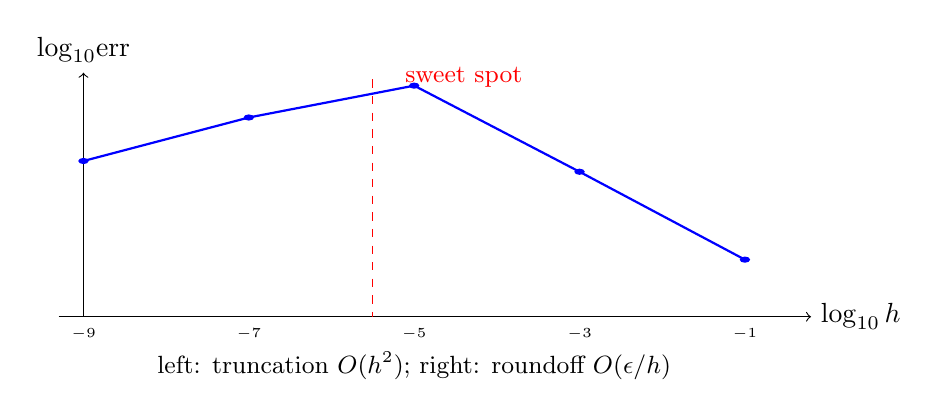
\begin{tikzpicture}[xscale=1.05,yscale=0.62]
\draw[->] (-9.3,0)--(-0.2,0) node[right]{$\log_{10}h$};
\draw[->] (-9,0)--(-9,5) node[above]{$\log_{10}$err};
% data: h=1e-1:2.486e-3->-2.6; 1e-3:2.486e-7->-6.6; 1e-5:3.0e-11->-10.5; 1e-7:8.5e-10->-9.07; 1e-9:8.2e-8->-7.09
% y = (-log10 err)*0.45 so lower err = higher point
\foreach \x/\e in {-1/2.60,-3/6.60,-5/10.52,-7/9.07,-9/7.09}{
  \fill[blue] (\x,{0.45*\e}) circle (1.8pt);}
\draw[blue,thick] (-1,{0.45*2.60})--(-3,{0.45*6.60})--(-5,{0.45*10.52})--(-7,{0.45*9.07})--(-9,{0.45*7.09});
\draw[dashed,red] (-5.5,{0.45*10.8})--(-5.5,0);
\node[red] at (-4.4,4.9) {\small sweet spot};
\node at (-5,-1.0) {\small left: truncation $O(h^2)$; right: roundoff $O(\epsilon/h)$};
\foreach \x/\l in {-1/{\(-1\)},-3/{\(-3\)},-5/{\(-5\)},-7/{\(-7\)},-9/{\(-9\)}}{\node at (\x,-0.35) {\tiny \l};}
\end{tikzpicture}

\caption{Finite-difference error vs.\ step size on the smooth function
(real data points from the listing output). Notice the U: truncation
$O(h^{2})$ on the left, roundoff on the right. Regenerate:
\ttfamily figures/ch11\_fd\_loglog.tex.}
\label{fig:fdlog}
\end{figure}

\begin{lstlisting}[caption={\ttfamily code/ch11\_sympy\_check.py ---
symbolic cross-check: SymPy confirms $\nabla\|Ax-b\|^2=2A^{T}(Ax-b)$
and the quadratic-form rule.}]
import sympy as sp

a11, a12, a21, a22 = sp.symbols('a11 a12 a21 a22')
x1, x2, b1, b2 = sp.symbols('x1 x2 b1 b2')
A = sp.Matrix([[a11, a12], [a21, a22]])
x = sp.Matrix([x1, x2]); b = sp.Matrix([b1, b2])
r = A * x - b
f = (r.T * r)[0]
print("f = ||Ax-b||^2 ="); print(sp.expand(f))
g = sp.Matrix([sp.diff(f, x1), sp.diff(f, x2)])
print("df/dx1 =", sp.expand(g[0]))
print("df/dx2 =", sp.expand(g[1]))
print("== 2*A.T*(A*x - b)?",
      sp.simplify(g - 2*A.T*(A*x - b)) == sp.zeros(2, 1))
# and the quadratic form x^T A x -> (A + A^T) x
A2 = sp.Matrix([[2, 1], [1, 3]])
q = (x.T * A2 * x)[0]
gq = sp.Matrix([sp.diff(q, x1), sp.diff(q, x2)])
print("grad x^T A x =", gq.T, " == 2Ax for symmetric A:",
      gq == 2*A2*x)
\end{lstlisting}

\begin{lstlisting}[caption={Output of the SymPy check --- the expanded
partial matches the matrix rule term for term, and the quadratic-form
identity verifies to \texttt{True}.}]
f = ||Ax-b||^2 =
a11**2*x1**2 + 2*a11*a12*x1*x2 - 2*a11*b1*x1 + a12**2*x2**2 - 2*a12*b1*x2 + a21**2*x1**2 + 2*a21*a22*x2 - 2*a21*b2*x1 + a22**2*x2**2 - 2*a22*b2*x2 + b1**2 + b2**2
df/dx1 = 2*a11**2*x1 + 2*a11*a12*x2 - 2*a11*b1 + 2*a21**2*x1 + 2*a21*a22*x2 - 2*a21*b2
df/dx2 = 2*a11*a12*x1 + 2*a12**2*x2 - 2*a12*b1 + 2*a21*a22*x1 + 2*a22**2*x2 - 2*a22*b2
== 2*A.T*(A*x - b)? True
grad x^T A x = Matrix([[4*x1 + 2*x2, 2*x1 + 6*x2]])  == 2Ax for symmetric A: True
\end{lstlisting}

\begin{lstlisting}[caption={\ttfamily code/ch11\_grad\_field.py --- the
data behind Figure~\ref{fig:gradcontour}: sampled gradients and the
gradient$\perp$tangent check.}]
import numpy as np
np.set_printoptions(precision=3, suppress=True)

# f = x^2 - x y + y^2, grad = (2x - y, -x + 2y); min at origin
def grad(v):
    x, y = v
    return np.array([2*x - y, -x + 2*y])

print("gradient field samples (position -> grad):")
for v in [np.array([1.,0.]), np.array([0.,1.]), np.array([1.,1.]),
          np.array([-1.,0.]), np.array([0.,-1.]), np.array([2.,1.])]:
    print(" ", v, "->", grad(v))
print("level sets: x^2 - xy + y^2 = c are ellipses;")
print("grad is normal to the level set everywhere (e.g. at (1,1)):")
v = np.array([1., 1.])
g = grad(v)
d = np.array([-g[1], g[0]])
print("  grad(1,1)=", g, " tangent dir=", d/np.linalg.norm(d),
      " dot=", np.dot(g, d/np.linalg.norm(d)))
\end{lstlisting}

\begin{lstlisting}[caption={Output of the field sampler. Notice
$\nabla f(1,1)\cdot\mathbf t=0$ exactly --- gradient perpendicular to
the level curve's tangent, numerically confirmed.}]
gradient field samples (position -> grad):
  [1. 0.] -> [ 2. -1.]
  [0. 1.] -> [-1.  2.]
  [1. 1.] -> [1. 1.]
  [-1.  0.] -> [-2.  1.]
  [ 0. -1.] -> [ 1. -2.]
  [2. 1.] -> [3. 0.]
level sets: x^2 - xy + y^2 = c are ellipses;
grad is normal to the level set everywhere (e.g. at (1,1)):
  grad(1,1)= [1. 1.]  tangent dir= [-0.707  0.707]  dot= 0.0
\end{lstlisting}

\begin{exercise}[easy]
Which of the library gradients is NOT defined componentwise, and why does
that matter for implementation?
\end{exercise}

\section{Hand derivation}\label{sec:handderiv11}

Derive $\nabla_{\mathbf x}(\mathbf x^{T}A\mathbf x)=(A+A^{T})\mathbf x$
--- the single most reused gradient in this book. Expand:
$\mathbf x^{T}A\mathbf x=\sum_{i,j}a_{ij}x_ix_j$. The $x_k$-derivative
collects terms where $i=k$ or $j=k$:
\[
\frac{\partial}{\partial x_k}\sum_{ij}a_{ij}x_ix_j
=\sum_j a_{kj}x_j+\sum_i a_{ik}x_i
=(A\mathbf x)_k+(A^{T}\mathbf x)_k.
\]
So $\nabla=(A+A^{T})\mathbf x$, and for symmetric $A$ the standard
$2A\mathbf x$. The SymPy listing verifies the same identity at
$A=\begin{bmatrix}2&1\\1&3\end{bmatrix}$ symbolically.

\section{Common mistakes}\label{sec:mvc-mistakes}

\begin{tripwire}[{Row-vs-column gradient layout}]
Some sources store $\partial f/\partial\mathbf x$ of a scalar as a
$1\times n$ row; this book stores $\nabla f$ as a column. Mixing them
transposes every downstream result --- often silently when dimensions
coincide. Pick one convention (ours: gradient is a column, Jacobian is
$m\times n$) and check shapes at every step.
\end{tripwire}

\begin{tripwire}[{Chain-rule multiplication order}]
$J_{f\circ g}=J_f\,J_g$ --- outer on the LEFT. Writing $J_gJ_f$ compiles
fine in index-free notation and is wrong; the shapes only commute when
the functions do, which is never.
\end{tripwire}

\begin{tripwire}[{Finite-difference step too large or too small}]
$h$ too big $\to$ truncation $O(h^{2})$; too small $\to$ roundoff
$O(\epsilon/h)$ swamps the slope. The U-curve of
Figure~\ref{fig:fdlog} is the diagnostic; $h\approx10^{-5}$ is the
default for float64.
\end{tripwire}

\begin{tripwire}[{``Derivative $\ne$ gradient $\ne$ steepest ascent'' wording trap}]
A partial derivative is a scalar; the gradient is their vector; the
steepest direction is that vector NORMALIZED. Sloppy wording silently
mixes a direction with a magnitude --- $\lVert\nabla f\rVert$ is the
slope, $\nabla f/\lVert\nabla f\rVert$ the direction.
\end{tripwire}

\begin{tripwire}[{Treating $\partial f/\partial\mathbf x$ of a scalar as a matrix}]
For scalar $f$ there is no matrix --- a $1\times n$ Jacobian row or the
$n\times1$ gradient column. ``The derivative of $f$ w.r.t.\ a matrix''
needs numerator/denominator layout conventions this book avoids by
design.
\end{tripwire}

\section{Summary}

\begin{center}
\begin{tabularx}{\textwidth}{l>{\raggedright\arraybackslash}X}
\toprule
\textbf{Object} & \textbf{What you need to know}\\
\midrule
Partial & ordinary derivative per axis; not the same as differentiability
\\
Gradient & column of partials; steepest ascent direction; normal to level
sets; $\lVert\nabla f\rVert$ = steepest slope \\
Directional deriv.\ & $\nabla f\cdot\mathbf d$ (unit $\mathbf d$) \\
Jacobian & $m\times n$ all-partials; local linear map: $F(x_0+\Delta)
\approx F(x_0)+J\Delta$ \\
Hessian & Jacobian of $\nabla f$, symmetric; eig = curvatures; $H\succ0$
$\Rightarrow$ min \\
Chain rule & $J_{f\circ g}=J_fJ_g$; $\nabla_x L=J_g^{T}\nabla_y L$ =
backprop \\
Library & $\mathbf w^{T}\mathbf x\to\mathbf w$; $\mathbf x^{T}A\mathbf
x\to(A+A^{T})\mathbf x$; $\|Ax-b\|^2\to2A^{T}(Ax-b)$; logits $\to$
softmax $-$ one-hot \\
FD check & central $(f(x{+}h){-}f(x{-}h))/2h$, $h{\approx}10^{-5}$; watch
the U-curve \\
\bottomrule
\end{tabularx}
\end{center}

\section*{Additional exercises}
\addcontentsline{toc}{section}{Additional exercises}

\begin{exercise}[easy]
All third-order partials of $f(x,y)=x^{3}y^{2}$ --- count them and compute
each.
\end{exercise}

\begin{exercise}[easy]
Gradient and Hessian of $f(\mathbf x)=\mathbf c^{T}\mathbf x$. When is a
linear function's Hessian informative?
\end{exercise}

\begin{exercise}[easy]
Evaluate $\nabla f$ of $f=x_1^{2}x_2+x_2e^{x_3}$ at $(1,2,0)$.
\end{exercise}

\begin{exercise}[easy]
Is the directional derivative linear in the direction? Prove or give a
counterexample.
\end{exercise}

\begin{exercise}[medium]
Derive $\nabla_{\mathbf w}\lVert\mathbf y-X\mathbf w\rVert^{2}$ by the
library rules alone (no index work) --- then connect to chapter 8's normal
equations.
\end{exercise}

\begin{exercise}[medium]
In code: verify the softmax cross-entropy gradient of the worked library
by finite differences on a 5-class example.
\end{exercise}

\begin{exercise}[medium]
Show the Hessian of $\mathbf x^{T}A\mathbf x$ is $A+A^{T}$; deduce the
quadratic $f$ has $H=2A$ when symmetric.
\end{exercise}

\begin{exercise}[medium]
Directional derivative of $f=x^{2}+y^{2}+z^{2}$ at $(1,2,2)$ along
$\mathbf d=(2,1,-2)/3$ --- compute via $\nabla f\cdot\mathbf d$ and
directly by 1-D calculus, and confirm equality.
\end{exercise}

\begin{exercise}[medium]
Show Clairaut can fail: state a function where mixed partials differ and
say which continuity hypothesis is violated.
\end{exercise}

\begin{exercise}[hard]
Derive the Hessian of the logistic loss
$\ell(\mathbf w)=\log(1+e^{-\mathbf w^{T}\mathbf x})$ and prove it is
PSD (the loss is convex).
\end{exercise}

\begin{exercise}[hard]
Two-layer chain rule by hand: for $\mathbf z=A_2\tanh(A_1\mathbf x)$,
scalar $L=\tfrac12\|z\|^2$, compute $\nabla_{A_1}L$ and $\nabla_{A_2}L$
as outer products of errors times activations --- the actual backprop
gradient.
\end{exercise}

\begin{exercise}[hard]
Implement second-order finite differences for the Hessian (four-point
formula) and check the Hessian of $f=x^{2}e^{y}$ at $(1,1)$ against the
analytic matrix.
\end{exercise}

\begin{exercise}[hard]
Prove: if $f$ is smooth and $\nabla f(\mathbf x_0)=0$ with $H(\mathbf
x_0)\succ0$, there is a neighbourhood where $f(\mathbf x)>f(\mathbf x_0)$
--- the second-order sufficient condition, via the SVD of $H$.
\end{exercise}

\section*{Notes}
\addcontentsline{toc}{section}{Notes}

\chapternotes{%
The gradient-library table and the matrix layout conventions follow MML
ch.~5 \cite{mml}, including the row-vs-column hazards its GitHub issues
flag; CS229's own prerequisite page \cite{cs229} is the external evidence
that this exact material is what a real ML course assumes on day one;
Kochenderfer ch.~2 \cite{koch} supplies the algorithm-first framing of
derivatives-as-tools; the contour pedagogy follows the 18.02 tradition of
drawing level sets before differentiating them.}
